\documentclass[b4paper, landscape, dvipdfmx]{jsarticle}
%----- 必要なパッケージ -----
\usepackage{fancybox,ascmac,otf}
\usepackage{amssymb, amsthm}
\usepackage[leqno]{amsmath}
\usepackage{geometry}
\usepackage{multicol}
\usepackage{tcolorbox}
\usepackage{xcolor}
\usepackage{fancyhdr}
\usepackage{tikz}

% TikZライブラリ
\usetikzlibrary{
    positioning,
    arrows.meta,
    calc,
    shadows,
    shadows.blur,
    intersections,
    angles,
    quotes
}

% tcolorboxライブラリ
\tcbuselibrary{skins, breakable, theorems}

\usepackage{enumitem}
\setlist[enumerate,1]{label=(\arabic*)}
\setlist[itemize]{leftmargin=*}
\newcommand{\ds}{\displaystyle}

%----- レイアウト設定 -----
\geometry{
  left=15mm,
  right=15mm,
  top=20mm,
  bottom=15mm,
  headheight=25pt
}

%----- 数式環境の上下の余白調整 -----
\AtBeginDocument{
  \setlength{\abovedisplayskip}{5pt}
  \setlength{\belowdisplayskip}{5pt}
  \setlength{\abovedisplayshortskip}{0pt}
  \setlength{\belowdisplayshortskip}{3pt}
}

%===========================================================
%  デザイン設定
%===========================================================

%--- 色の定義 ---
\definecolor{printBlue}{RGB}{0, 50, 100}     % 濃紺
\definecolor{printRed}{RGB}{140, 20, 20}     % 濃エンジ
\definecolor{printTeal}{RGB}{0, 60, 60}      % 濃い青緑

%--- 共通スタイル定義 ---
\tcbset{
    chartbox/.style={
        enhanced,
        fonttitle=\sffamily\bfseries,
        boxrule=1pt,
        arc=2pt,
        top=1.0em,
        nobeforeafter,
        enlarge left by=-2mm,
        enlarge right by=-2mm,
        drop fuzzy shadow,
        colback=white,
        attach boxed title to top left={xshift=10pt, yshift*=-\tcboxedtitleheight/2},
        boxed title style={frame hidden, sharp corners, rounded corners=southeast, arc=3pt}
    }
}

%--- 各種ボックス環境定義 ---

% セクション・枠組み用 (any)
\newtcolorbox{any}[1]{
    enlarge left by=0mm, enlarge right by=0mm,
    enhanced, frame hidden, colback=white, title={#1},
    attach boxed title to top left={xshift=0mm, yshift=0mm},
    coltitle=white, fonttitle=\bfseries\sffamily,
    boxed title style={
        colback=black!80, frame hidden, arc=4pt, outer arc=4pt,
        sharp corners=south, boxrule=0pt,
        top=1mm, bottom=1mm, left=3mm, right=3mm
    },
    underlay boxed title={
        \draw[thick, black!80] (title.south west) -- (title.south west-|frame.east);
    },
    breakable, top=5mm, left=2mm, right=2mm, bottom=0mm,
    before skip=1em, after skip=1em,
    segmentation style={draw=black!40, dashed}
}

% 例題 (eg)
\newtcolorbox{eg}[1]{
    chartbox,
    colframe=printBlue,
    coltitle=white,
    title=\textbf{例題 #1},
    boxed title style={colback=printBlue},
    segmentation style={draw=printBlue, line width=0.5pt, dashed}
}

% 練習 (prac)
\newtcolorbox{prac}[1]{
    chartbox,
    colframe=printRed,
    coltitle=white,
    title=\textbf{練習 #1},
    boxed title style={colback=printRed}
}

% 定理 (thm)
\newtcolorbox{thm}[1]{
    chartbox,
    colframe=printTeal,
    coltitle=white,
    title=\textbf{#1},
    boxed title style={colback=printTeal}
}

% 解答欄 (answer)
\newtcolorbox{answer}[1][height fill]{
    enhanced,
    title={Memo / Answer},
    colframe=black!80,
    colback=white,
    coltitle=black!60,
    fonttitle=\sffamily\bfseries,
    attach boxed title to top left={xshift=5mm, yshift*=-\tcboxedtitleheight/2},
    boxed title style={frame hidden, colback=white},
    boxrule=1pt,
    arc=1pt,
    nobeforeafter,
    enlarge left by=-2mm, 
    enlarge right by=-2mm, 
    height fill,
    segmentation style={draw=black!20, solid},
    underlay={
        \begin{tcbclipinterior}
            \draw[step=5mm, black!5, ultra thin] (interior.south west) grid (interior.north east);
        \end{tcbclipinterior}
    }, 
    #1
}

%----- 段組の設定 -----
\setlength{\columnsep}{15mm}
\setlength{\columnseprule}{0.4pt}
\renewcommand{\columnseprulecolor}{\color{black!30}}

%----- ヘッダーの設定 -----
\pagestyle{fancy}
\fancyhf{}
\fancyhead[C]{%
    \begin{tikzpicture}[remember picture, overlay]
        \node[anchor=north west, fill=printBlue, minimum width=\paperwidth, minimum height=5pt] at (current page.north west) {};
    \end{tikzpicture}
}
\fancyhead[L]{\small \textcolor{black!90}{数学C $>$ 第1章--平面ベクトル $>$ 第6回 \textbf{内積の演算と等式の証明}}}
\fancyhead[R]{\small 年 \hspace{1cm} 組 \hspace{1cm} 番 \quad 氏名 \hspace{6cm}}
\renewcommand{\headrulewidth}{0pt}

\begin{document}

%=============================================================================
% 1枚目:大きさの計算(展開公式)
%=============================================================================
\begin{multicols}{2}

%-----------------------------------------------------------------------------
% 左カラム:大きさの2乗と展開
%-----------------------------------------------------------------------------
\begin{any}{1. ベクトルの「大きさ」の扱い方}
    ベクトルの大きさ $|\vec{a}|$ は, そのままでは扱いにくい.
    しかし, \textbf{2乗すると内積に変身する}という最強の性質がある.

    \begin{thm}{大きさの2乗公式}
        同じベクトル同士の内積は, 大きさの2乗になる.
        \[ \vec{a} \cdot \vec{a} = |\vec{a}| |\vec{a}| \cos 0^\circ = |\vec{a}|^2 \]
        逆に, 大きさ $|\vec{a}|$ が出てきたら, \textbf{とりあえず2乗して内積に持ち込む}のが定石である.
    \end{thm}

    \begin{thm}{ベクトルの展開公式}
        ベクトルの内積は分配法則が成り立つため, 文字式の展開(乗法公式)と同じ感覚で計算できる.
        
        \begin{enumerate}
            \item $|\vec{a} + \vec{b}|^2 = (\vec{a} + \vec{b}) \cdot (\vec{a} + \vec{b}) = |\vec{a}|^2 + 2\vec{a}\cdot\vec{b} + |\vec{b}|^2$
            \item $|\vec{a} - \vec{b}|^2 = |\vec{a}|^2 - 2\vec{a}\cdot\vec{b} + |\vec{b}|^2$
            \item $(\vec{a} + \vec{b}) \cdot (\vec{a} - \vec{b}) = |\vec{a}|^2 - |\vec{b}|^2$
        \end{enumerate}
        \textbf{注意:} $2\vec{a}\cdot\vec{b}$ の部分は単なる掛け算ではなく「内積」である.
    \end{thm}

    \begin{eg}{1 (基本計算)}
        $|\vec{a}|=3, |\vec{b}|=2$, なす角が $60^\circ$ とする.
        このとき, $|\vec{a} + 2\vec{b}|$ の値を求めよ.
        \tcblower
        \textbf{手順:}
        1. まず内積 $\vec{a}\cdot\vec{b}$ を求めておく.
        2. 求めたい式を\textbf{2乗して展開}する.
        3. 最後にルートをとる.
        \vspace{3cm}
    \end{eg}
\end{any}

%-----------------------------------------------------------------------------
% 右カラム:計算練習
%-----------------------------------------------------------------------------
\columnbreak

\begin{eg}{2 (垂直と実数倍)}
    $|\vec{a}|=2, |\vec{b}|=1$, なす角が $120^\circ$ とする.
    ベクトル $\vec{a} + t\vec{b}$ が $\vec{b}$ と垂直になるとき, 実数 $t$ の値を求めよ.
    
    \tcblower
    \textbf{ヒント:} 「垂直」 $\iff$ 「内積が 0」.
    \[ (\vec{a} + t\vec{b}) \cdot \vec{b} = 0 \]
    この式を展開して計算する.
    \vspace{8cm}
\end{eg}

\end{multicols}

%=============================================================================
% 2枚目:等式の証明
%=============================================================================
\newpage
\begin{multicols}{2}

%-----------------------------------------------------------------------------
% 左カラム:幾何学的証明
%-----------------------------------------------------------------------------
\begin{any}{2. 等式の証明と図形的意味}
    ベクトルの演算性質を利用して, 図形の定理を証明できる.
    
    \begin{eg}{3 (中線定理の証明)}
        $\triangle ABC$ において, 辺BCの中点をMとする. このとき,
        \[ AB^2 + AC^2 = 2(AM^2 + BM^2) \]
        が成り立つことをベクトルを用いて証明せよ.
        
        \tcblower
        \textbf{証明の方針:}
        始点をMにそろえる(位置ベクトル).
        $\overrightarrow{\text{MB}}, \overrightarrow{\text{MC}}$ は長さが等しく逆向きなので...
        \begin{center}
        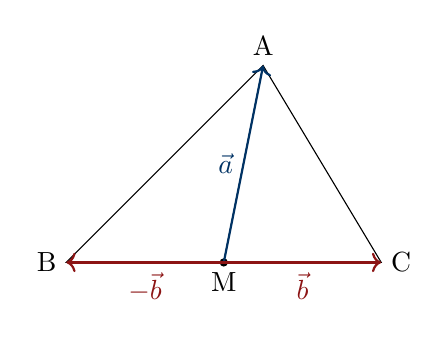
\begin{tikzpicture}[scale=1]
            \coordinate (M) at (0,0);
            \coordinate (B) at (-2,0);
            \coordinate (C) at (2,0);
            \coordinate (A) at (0.5, 2.5);
            
            \draw (A)--(B)--(C)--cycle;
            \draw (A)--(M);
            \fill (M) circle (1.5pt) node[below] {M};
            \node[above] at (A) {A};
            \node[left] at (B) {B};
            \node[right] at (C) {C};
            
            % vector notation
            \draw[->, thick, printBlue] (M)--(A) node[midway, left] {$\vec{a}$};
            \draw[->, thick, printRed] (M)--(C) node[midway, below] {$\vec{b}$};
            \draw[->, thick, printRed] (M)--(B) node[midway, below] {$-\vec{b}$};
        \end{tikzpicture}
        \end{center}
        \vspace{8cm}
    \end{eg}
\end{any}

%-----------------------------------------------------------------------------
% 右カラム:平行四辺形の法則
%-----------------------------------------------------------------------------
\columnbreak

\begin{any}{3. 平行四辺形の法則}
    \begin{thm}{平行四辺形の法則}
        平行四辺形の対角線の長さについて, 以下の等式が成り立つ.
        \[ |\vec{a}+\vec{b}|^2 + |\vec{a}-\vec{b}|^2 = 2(|\vec{a}|^2 + |\vec{b}|^2) \]
        (対角線の長さの2乗和)=(各辺の長さの2乗和)
    \end{thm}
    
    \begin{center}
    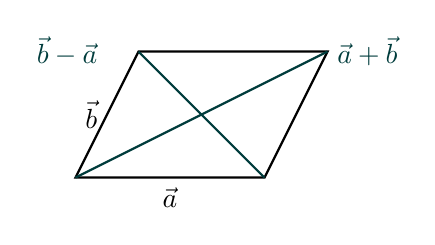
\begin{tikzpicture}[scale=0.8, >=stealth]
        \coordinate (O) at (0,0);
        \coordinate (A) at (3,0);
        \coordinate (B) at (1,2);
        \coordinate (C) at (4,2);
        
        \draw[thick] (O)--(A)--(C)--(B)--cycle;
        \draw[thick, printTeal] (O)--(C);
        \draw[thick, printTeal] (A)--(B);
        
        \node[below] at (1.5,0) {$\vec{a}$};
        \node[left] at (0.5,1) {$\vec{b}$};
        \node[right, printTeal] at (4,2) {$\vec{a}+\vec{b}$};
        \node[left, printTeal] at (0.5,2) {$\vec{b}-\vec{a}$};
    \end{tikzpicture}
    \end{center}

    この証明は, 左辺を展開して整理するだけで完了する.
    
    \begin{answer}[height=10cm]
    \end{answer}
\end{any}

\end{multicols}

%=============================================================================
% 3枚目:確認テスト(問題)
%=============================================================================
\newpage
\fancyhead[L]{\small \textcolor{black!90}{数学C $>$ 第1章--平面ベクトル $>$ 第6回--\textbf{確認テスト}}}
\begin{multicols}{2}

\begin{any}{確認テスト (A: 基本)}
    \begin{prac}{A1 (大きさの計算)}
        $|\vec{a}|=2, |\vec{b}|=3, \vec{a}\cdot\vec{b}=-3$ とする.
        \begin{enumerate}
            \item $|\vec{a} + \vec{b}|^2$ を求めよ.
            \item $|\vec{a} - \vec{b}|$ を求めよ.
        \end{enumerate}
    \end{prac}
    \begin{answer}[height=5cm]
    \end{answer}

    \begin{prac}{A2 (垂直なベクトル)}
        $|\vec{a}|=1, |\vec{b}|=2$, なす角 $60^\circ$ とする.
        $\vec{a} + t\vec{b}$ と $\vec{a} - \vec{b}$ が垂直であるとき, 実数 $t$ の値を求めよ.
    \end{prac}
    \begin{answer}[height=5cm]
    \end{answer}
\end{any}

\columnbreak

\begin{any}{確認テスト (B: 標準)}
    \begin{prac}{B1 (ベクトルの大きさ)}
        2つのベクトル $\vec{a}, \vec{b}$ が,
        \[ |\vec{a}+\vec{b}| = 4, \quad |\vec{a}-\vec{b}| = 2 \]
        を満たすとき, 内積 $\vec{a}\cdot\vec{b}$ の値を求めよ.
    \end{prac}
    \begin{answer}[height=6cm]
    \end{answer}

    \begin{prac}{B2 (大きさの最小値)}
        $|\vec{a}|=2, |\vec{b}|=2, \vec{a}\cdot\vec{b}=2$ とする.
        $|\vec{a} + t\vec{b}|$ が最小となるときの実数 $t$ の値と, その最小値を求めよ.
        \vspace{0.5em}
        \\
        \textbf{ヒント:} 2乗して $t$ の2次関数として扱う.
    \end{prac}
    \begin{answer}[height=6cm]
    \end{answer}
\end{any}

\end{multicols}

%=============================================================================
% 4枚目:確認テスト(解答)
%=============================================================================
\newpage
\fancyhead[L]{\small \textcolor{black!90}{数学C $>$ 第1章--平面ベクトル $>$ 第6回 \textbf{【解答解説】}}}

\begin{multicols}{2}

\begin{any}{解答 (A: 基本)}
    \begin{answer}[height=8cm]
    \color{printRed}
    \textbf{A1 (解答)}
        (1) 展開公式を利用する.
        \begin{align*}
            |\vec{a} + \vec{b}|^2 &= |\vec{a}|^2 + 2\vec{a}\cdot\vec{b} + |\vec{b}|^2 \\
            &= 2^2 + 2(-3) + 3^2 \\
            &= 4 - 6 + 9 = \boldsymbol{7}
        \end{align*}
        
        (2) 同様に2乗して計算する.
        \begin{align*}
            |\vec{a} - \vec{b}|^2 &= |\vec{a}|^2 - 2\vec{a}\cdot\vec{b} + |\vec{b}|^2 \\
            &= 4 - 2(-3) + 9 \\
            &= 4 + 6 + 9 = 19
        \end{align*}
        大きさは正なので, $|\vec{a} - \vec{b}| = \boldsymbol{\sqrt{19}}$
    \end{answer}

    \begin{answer}[height=8cm]
    \color{printRed}
    \textbf{A2 解答:} \\
    まず内積の準備: $\vec{a}\cdot\vec{b} = 1 \cdot 2 \cdot \cos 60^\circ = 1$.
    
    垂直条件より, 内積が0.
    \begin{align*}
        (\vec{a} + t\vec{b}) \cdot (\vec{a} - \vec{b}) &= 0 \\
        |\vec{a}|^2 - \vec{a}\cdot\vec{b} + t\vec{a}\cdot\vec{b} - t|\vec{b}|^2 &= 0 \\
        1^2 - 1 + t(1) - t(2^2) &= 0 \\
        1 - 1 + t - 4t &= 0 \\
        -3t &= 0 \\
        \therefore \quad t &= 0
    \end{align*}
    (注: 計算結果が0になることもある)
    \end{answer}
\end{any}

\columnbreak

\begin{any}{解答 (B: 標準)}
    \begin{answer}[height=6cm]
    \color{printRed}
    \textbf{B1 解答:} \\
    与えられた条件をそれぞれ2乗する.
    \begin{itemize}
        \item $|\vec{a}+\vec{b}|^2 = 16 \implies |\vec{a}|^2 + 2\vec{a}\cdot\vec{b} + |\vec{b}|^2 = 16 \dots (1)$
        \item $|\vec{a}-\vec{b}|^2 = 4 \implies |\vec{a}|^2 - 2\vec{a}\cdot\vec{b} + |\vec{b}|^2 = 4 \dots (2)$
    \end{itemize}
    $(1) - (2)$ を計算すると, $|\vec{a}|^2, |\vec{b}|^2$ が消える.
    \begin{align*}
        4\vec{a}\cdot\vec{b} &= 12 \\
        \vec{a}\cdot\vec{b} &= \boldsymbol{3}
    \end{align*}
    \end{answer}

    \begin{answer}[height fill]
    \color{printRed}
    \textbf{B2 解答:} \\
    $y = |\vec{a} + t\vec{b}|^2$ とおき, 最小値を考える.
    \begin{align*}
        y &= |\vec{a}|^2 + 2t\vec{a}\cdot\vec{b} + t^2|\vec{b}|^2 \\
        &= 4 + 2t(2) + t^2(4) \\
        &= 4t^2 + 4t + 4
    \end{align*}
    これを平方完成する.
    \begin{align*}
        y &= 4(t^2 + t) + 4 \\
        &= 4(t + \frac{1}{2})^2 - 1 + 4 \\
        &= 4(t + \frac{1}{2})^2 + 3
    \end{align*}
    よって $t = -\frac{1}{2}$ のとき, 最小値 3 をとる... \textbf{ではない!}
    
    求めているのは $|\vec{a} + t\vec{b}|$ (2乗する前)の最小値なので,
    $y$ の最小値のルートをとる必要がある.
    
    \textbf{答え:}
    $t = -\frac{1}{2}$ のとき, 最小値 $\sqrt{3}$
    \end{answer}
\end{any}

\end{multicols}
\end{document}